%!TEX root = Main.tex
\documentclass[Main]{subfiles}

\begin{document}



\subsection{Class diagrams}
In Figure \ref{fig:wrapperfacadeuml} the interaction between the classes that form the server can be seen. 
It should be noted, that not every class have been added with their methods. 
This has been done to decrease the complexity of the tree and to only show the interesting parts of the system.
Therefore only the interface, \code{Event\_handler}, has the methods and thus the the interesting parts of the realizations can be found in the interface.
Furthermore the classes that is part of the WrapperFacade- (\code{SOCK\_Stream} and \code{SOCK\_Acceptor}) and the Reactor pattern, (\code{Reactor}), are described in section \ref{sec:patterns}\fxnote{What is described there now?}.

\begin{figure}[hbtp]
\centering
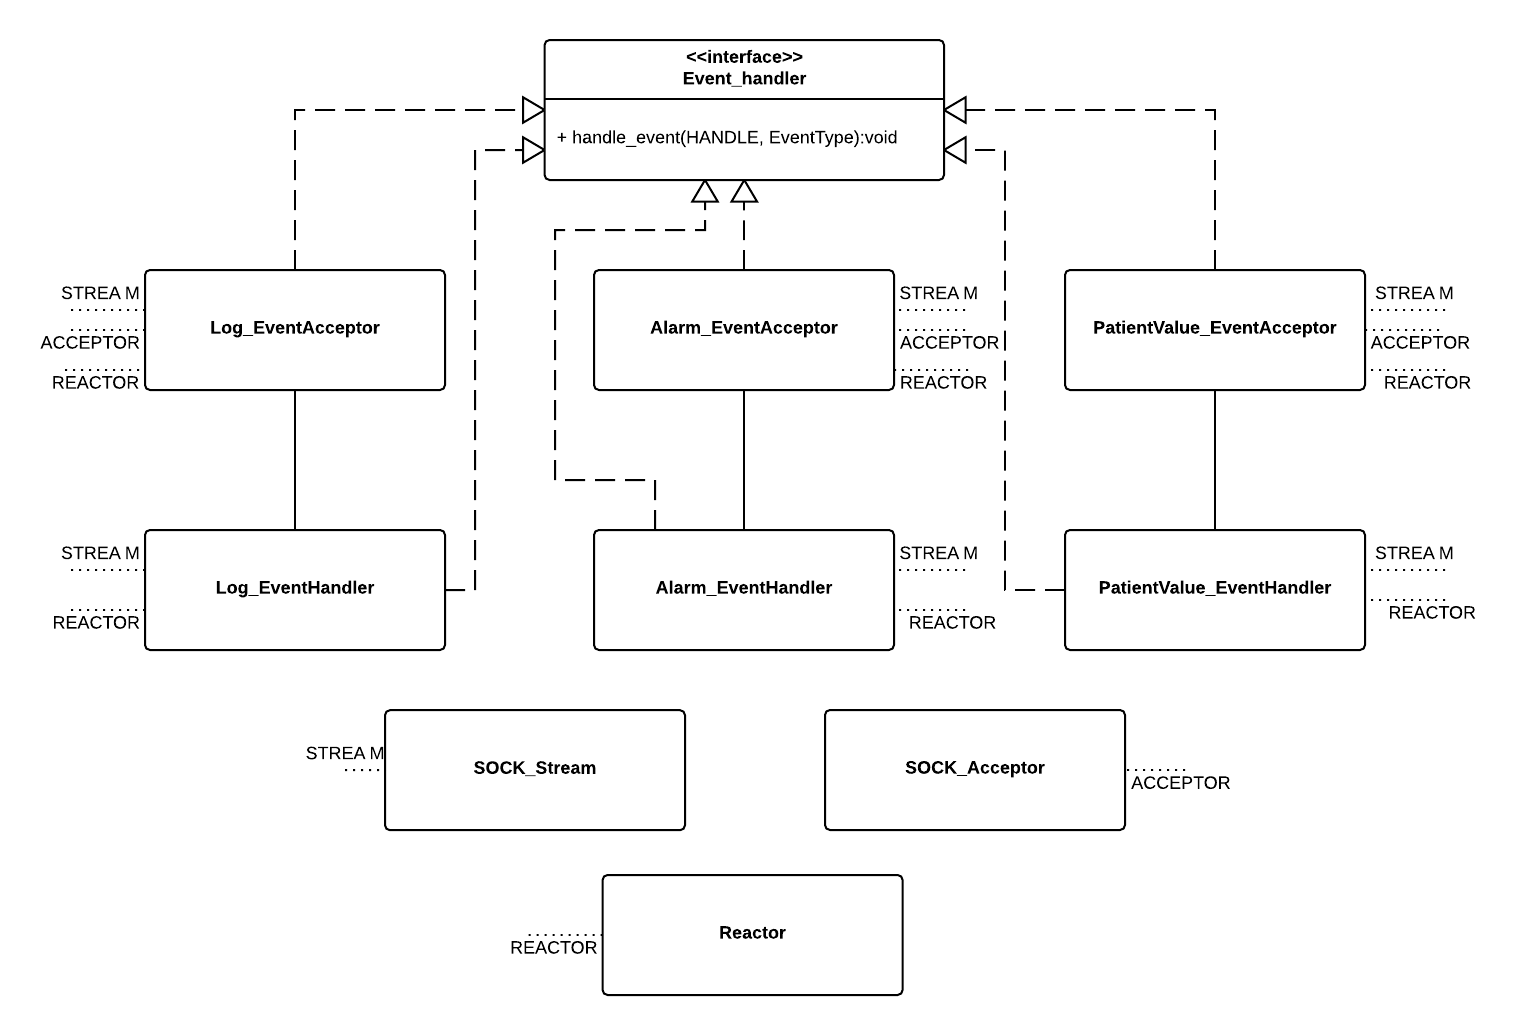
\includegraphics[width=1.0\textwidth]{ServerClassDiagram}
\caption{Class diagram for the classes that interact to form the server}
\label{fig:wrapperfacadeuml}
\end{figure}


\end{document}